\section{Results}
\label{sec:results}

\subsection{The two-stage loop does not converge}
\label{sec:primary}

\begin{table}[t]
    \centering
    \resizebox{\textwidth}{!}{%
    \begin{tabular}{@{}lccccccc@{}}
        \toprule
        \textbf{Condition} & \textbf{mean final $\Delta$} & \textbf{clean min $\Delta^{\dagger}$} & \textbf{\% exact FP} & \textbf{\% approx FP} & \textbf{fit floor $c$} & \textbf{fit $R^2$} & \textbf{mean trunc.\ versions} \\
        \midrule
        \texttt{D1\_main} (two-stage)   & 0.376 & 0.340 & 0.00 & 0.00 & 0.307 & 0.61 & 3.9 \\
        \texttt{D2\_single\_stage}      & \textbf{0.048} & \textbf{0.046} & \textbf{0.08} & \textbf{0.42} & \textbf{0.048} & \textbf{0.98} & \textbf{0.0} \\
        \texttt{D2\_temp\_default}      & 0.601 & 0.567 & 0.00 & 0.00 & 0.455 & 0.27 & 4.2 \\
        \texttt{D2\_cross\_model}       & 0.228 & 0.234 & 0.00 & 0.00 & 0.250 & 0.79 & 2.8 \\
        \texttt{D2\_framing\_harsh}     & 0.451 & 0.453 & 0.00 & 0.00 & 0.324 & 0.57 & 5.2 \\
        \texttt{D2\_framing\_lenient}   & 0.245 & 0.218 & 0.00 & 0.00 & 0.244 & 0.77 & 2.9 \\
        \texttt{D2\_genre\_prose}       & 0.275 & 0.289 & 0.00 & 0.00 & 0.170 & 0.83 & 2.4 \\
        \texttt{D2\_unconstrained}      & 0.399 & 0.473 & 0.00 & 0.00 & 0.384 & 0.52 & 5.4 \\
        \bottomrule
    \end{tabular}
    }
    \caption{Convergence outcomes across conditions. The approximate-fixed-point (FP) threshold
    is $0.02$. Every two-stage condition sits an order of magnitude above it and reaches
    \emph{zero} exact and approximate fixed points; the fit floor $c$ is large and positive
    (relaxation toward non-zero churn). Only the single-stage baseline converges (bold): it
    decays to $c\approx 0.05$ with $R^2=0.98$ and reaches an approximate fixed point in $42\%$
    of documents.
    $^{\dagger}$\emph{clean min $\Delta$} is the smallest per-step $\Delta$ over
    truncation-free steps (robustness check).}
    \label{tab:main_results}
\end{table}


\tabref{tab:main_results} reports convergence outcomes for all eight conditions. Every
two-stage condition sits an order of magnitude above the $0.02$ approximate-fixed-point
threshold and never reaches it: \textbf{$0\%$ exact and $0\%$ approximate} fixed points
across the board. For \texttt{D1\_main}, the exponential fit leaves a large positive floor
$c\approx 0.31$---the process relaxes toward a \emph{moving, non-zero} level of churn, not
toward zero. The single-stage baseline, by contrast, decays cleanly to $c\approx 0.05$ with
$R^2=0.98$ and reaches an approximate fixed point in $42\%$ of documents, replicating
\citet{wu2026converge} and confirming that our harness detects convergence when it exists.

\Figref{fig:delta} makes the contrast concrete. The two-stage $\dt$ curve falls from $0.64$
to a plateau near $0.38$ by step 3 and stays there; the single-stage curve decays smoothly to
$\approx 0.05$; and at default temperature the curve oscillates in the $0.58$--$0.70$ band
with no relaxation at all.

\begin{figure}[t]
    \centering
    \begin{subfigure}[b]{0.48\textwidth}
        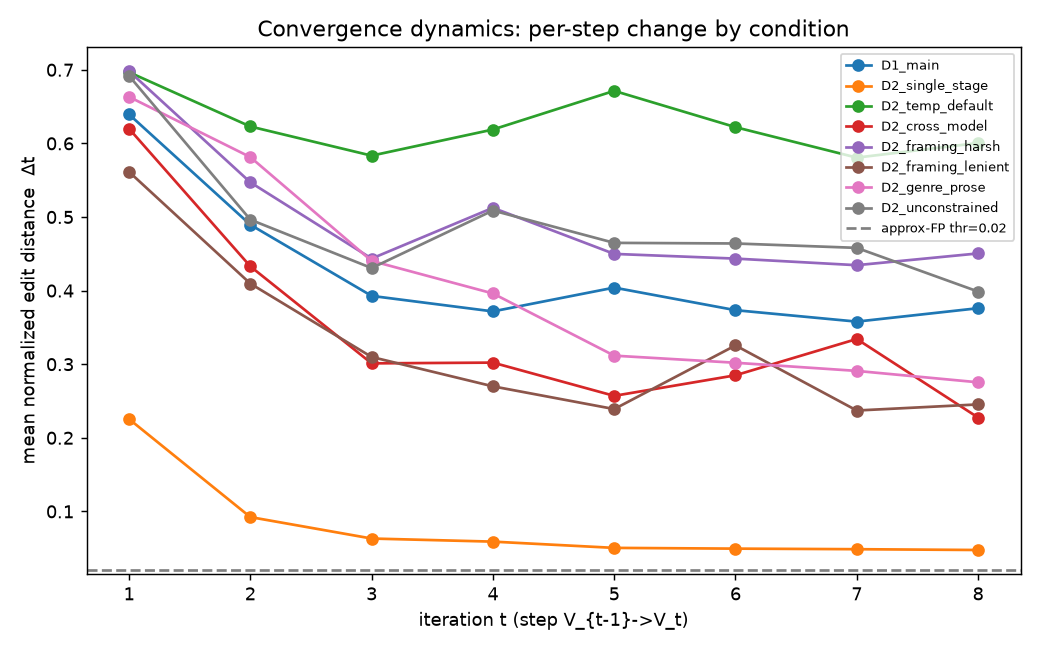
\includegraphics[width=\textwidth]{figures/delta_curves.png}
        \caption{Per-step edit distance $\dt$ over iterations.}
        \label{fig:delta}
    \end{subfigure}\hfill
    \begin{subfigure}[b]{0.48\textwidth}
        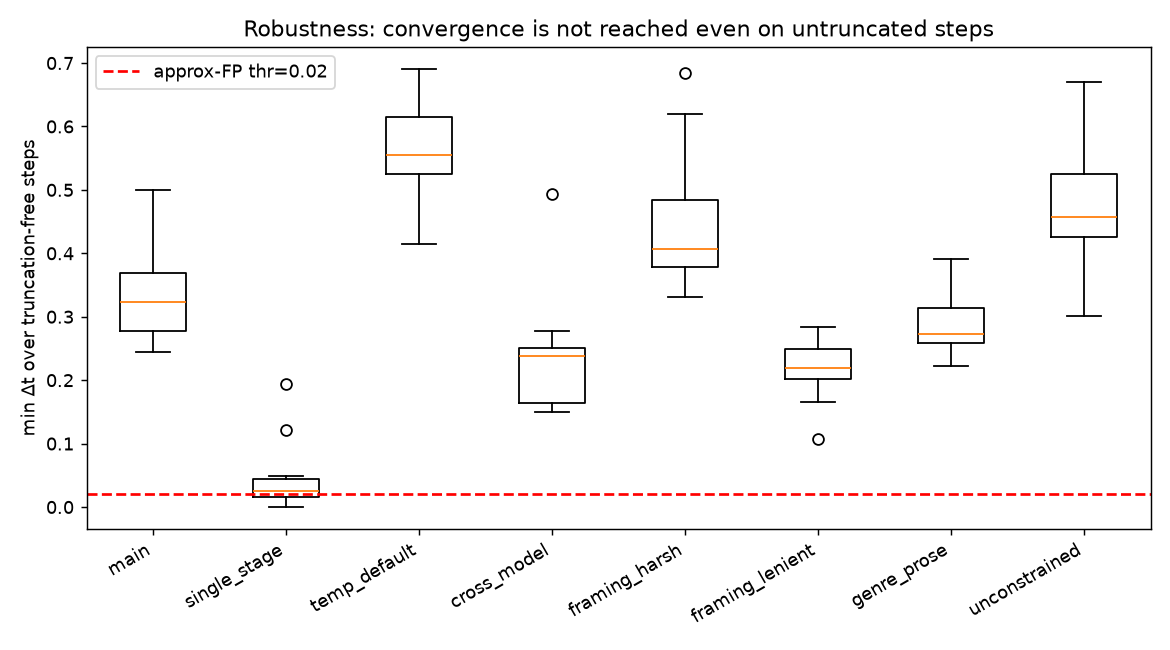
\includegraphics[width=\textwidth]{figures/clean_min_delta_box.png}
        \caption{Clean min $\Delta$ (truncation-free steps).}
        \label{fig:cleanmin}
    \end{subfigure}
    \caption{Convergence dynamics. \captiona\ The two-stage \twostage loop
    (\texttt{D1\_main}) plateaus near $0.38$; the single-stage \singlestage baseline decays to
    $\approx 0.05$; default temperature oscillates without relaxing. The dashed line marks the
    $0.02$ approximate-fixed-point threshold. \captionb\ Even the smallest per-step change over
    truncation-free steps stays far above the threshold for every two-stage condition, so
    non-convergence is not a truncation artifact.}
    \label{fig:convergence}
\end{figure}

\para{Statistical tests.} The result is highly significant. For \texttt{D1\_main}, final
$\Delta$ differs from $0$ with $t(11)=11.30$, $p=2.2\times10^{-7}$, and the truncation-free
clean min $\Delta$ differs from the $0.02$ threshold with $t(11)=13.01$,
$p=5.1\times10^{-8}$ (\figref{fig:cleanmin}): non-convergence survives the truncation control.
The single- vs.\ two-stage comparison, paired on the same documents, gives Wilcoxon
$p=4.9\times10^{-4}$ with \textbf{Cohen's $d_z=-3.26$} on clean min $\Delta$ ($d_z=-2.56$ on
final $\Delta$)---the dominant effect in the study.

\subsection{Determinants of (non-)convergence}
\label{sec:ablations}

\begin{table}[t]
    \centering
    \resizebox{\textwidth}{!}{%
    \begin{tabular}{@{}lcccl@{}}
        \toprule
        \textbf{Ablation (vs.\ \texttt{D1\_main})} & \textbf{direction} & \textbf{effect (Cohen's $d_z$)} & \textbf{$p$} & \textbf{reading} \\
        \midrule
        single-stage vs.\ two-stage        & $\downarrow\downarrow\downarrow$ converges & $-2.56$ & $5\times10^{-4}$ & \textbf{the} decisive factor \\
        temperature $1.0$ vs.\ $0$         & $\uparrow$ more churn / chaotic & $+2.09$ & $5\times10^{-4}$ & default temp destroys even relaxation ($R^2{=}0.27$) \\
        cross-model reviewer vs.\ self     & $\downarrow$ less churn & $-1.17$ & $5\times10^{-3}$ & a different reviewer eases pressure, still no FP \\
        lenient vs.\ structured framing    & $\downarrow$ less churn & $-1.14$ & $7\times10^{-3}$ & less to fix $\Rightarrow$ smaller edits, still no FP \\
        harsh vs.\ structured framing      & $\uparrow$ (n.s.) & $+0.45$ & $0.13$ & trend toward more churn \\
        unconstrained vs.\ length-preserving & $\uparrow$ (n.s.) & $+0.19$ & $0.62$ & length guidance barely helps \\
        \bottomrule
    \end{tabular}
    }
    \caption{Determinants of (non-)convergence: paired comparisons against \texttt{D1\_main}
    (Wilcoxon on final $\Delta$). No manipulation produces convergence; the single- vs.\
    two-stage contrast dominates every within-two-stage factor. Negative $d_z$ means less
    churn than \texttt{D1\_main}. n.s.\ = not significant.}
    \label{tab:ablations}
\end{table}


\tabref{tab:ablations} reports the seven-way ablation. \textbf{No manipulation produces
convergence.} The dynamics are modulated---a cross-model or lenient reviewer roughly
\emph{halves} the residual churn (final $\Delta$ from $0.376$ to $0.228$ and $0.245$
respectively), while a higher temperature makes it \emph{worse} and non-monotone (final
$\Delta=0.601$, fit $R^2=0.27$)---but the fixed point is never reached. Reviewer identity,
framing, and temperature tune the \emph{rate} of churn; only the presence or absence of the
review stage changes its \emph{existence}. Length guidance is nearly inert: unconstrained vs.\
length-preserving is not significant ($p=0.62$), a point we return to below.

\subsection{Mechanism: runaway inflation drives drift, not fidelity}
\label{sec:mechanism}

\begin{table}[t]
    \centering
    \begin{minipage}[t]{0.48\textwidth}
        \centering
        \resizebox{\textwidth}{!}{%
        \begin{tabular}{@{}lccc@{}}
            \toprule
            \textbf{Condition} & \textbf{$V_0$} & \textbf{$V_8$} & \textbf{growth} \\
            \midrule
            \texttt{D2\_single\_stage} & 1469 & 1519 & \textbf{1.03$\times$} \\
            \texttt{D1\_main}          & 1469 & 9869 & 6.72$\times$ \\
            \texttt{D2\_temp\_default} & 1469 & 9340 & 6.36$\times$ \\
            \texttt{D2\_unconstrained} & 1469 & 10478 & 7.13$\times$ \\
            \texttt{D2\_genre\_prose}  & 703  & 10380 & \textbf{14.8$\times$} \\
            \bottomrule
        \end{tabular}
        }
        \caption{Mean document length (characters), $V_0\to V_8$. The single-stage loop holds
        length; every two-stage loop explodes it. Length-preserving \texttt{D1\_main} is
        indistinguishable from unconstrained \texttt{D2\_unconstrained} ($p=0.62$): review
        pressure overrides the length instruction.}
        \label{tab:length}
    \end{minipage}\hfill
    \begin{minipage}[t]{0.48\textwidth}
        \centering
        \resizebox{\textwidth}{!}{%
        \begin{tabular}{@{}lcccc@{}}
            \toprule
            \textbf{Condition} & \textbf{$\cos(V_0,V_f)$} & \textbf{mean.\ /10} & \textbf{+cl.} & \textbf{--cl.} \\
            \midrule
            \texttt{D2\_single\_stage} & \textbf{0.973} & \textbf{10.0} & 0.0 & 0.0 \\
            \texttt{D1\_main}          & 0.769 & 6.2 & 4.2 & 2.1 \\
            \texttt{D2\_framing\_harsh}& 0.735 & 4.8 & 8.4 & 3.6 \\
            \texttt{D2\_genre\_prose}  & 0.627 & 4.8 & 15.5 & 1.6 \\
            \bottomrule
        \end{tabular}
        }
        \caption{Fidelity of $V_\text{final}$ vs.\ $V_0$: cosine similarity, LLM-judged
        meaning preservation (/10), and added/dropped claim counts (+cl.\ / --cl.). Inflation
        breaks fidelity: two-stage loops drift and fabricate claims, while single-stage
        preserves meaning perfectly.}
        \label{tab:fidelity}
    \end{minipage}
\end{table}


\para{Length explodes.} \tabref{tab:length} tracks mean document length from $V_0$ to $V_8$.
The single-stage loop holds length ($1.03\times$); every two-stage loop explodes it, with
\texttt{D1\_main} inflating $6.72\times$---a $1.5$\,KB abstract becomes a $\sim 10$\,KB
mini-paper (\figref{fig:length}). Crucially, the length-preserving instruction (``keep roughly
the same length'') is largely \emph{ignored} under review pressure: \texttt{D1\_main} (with the
instruction) is statistically indistinguishable from \texttt{D2\_unconstrained} (without it,
$7.13\times$; $p=0.62$). The review stage's steady demand for ``more precision / examples /
discussion'' overrides the length constraint.

\begin{figure}[t]
    \centering
    \begin{subfigure}[b]{0.32\textwidth}
        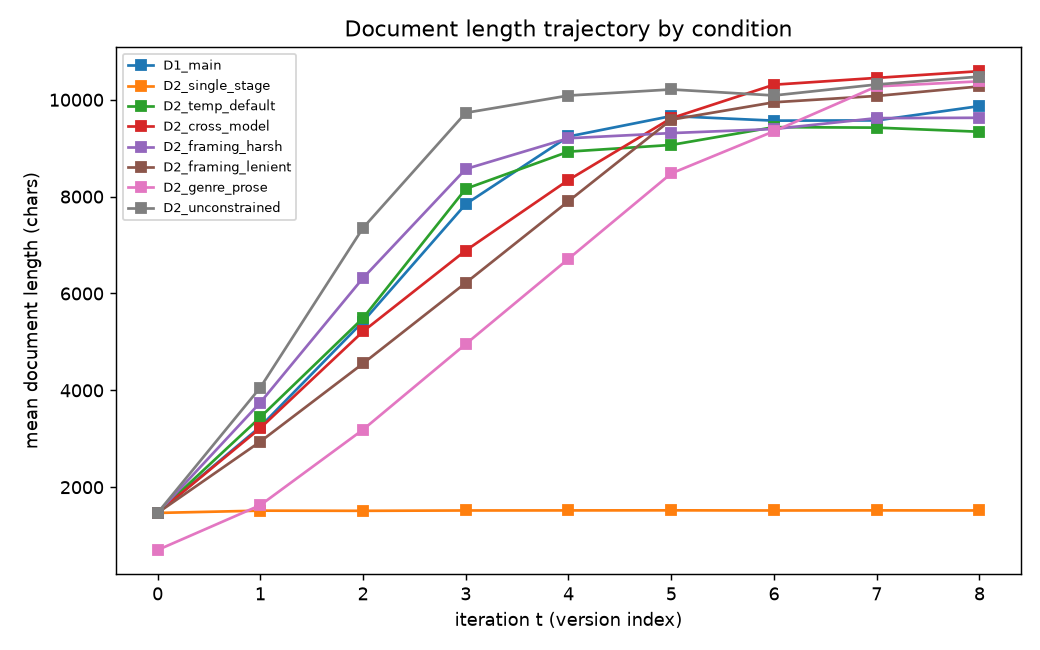
\includegraphics[width=\textwidth]{figures/length_growth.png}
        \caption{Document length}
        \label{fig:length}
    \end{subfigure}\hfill
    \begin{subfigure}[b]{0.32\textwidth}
        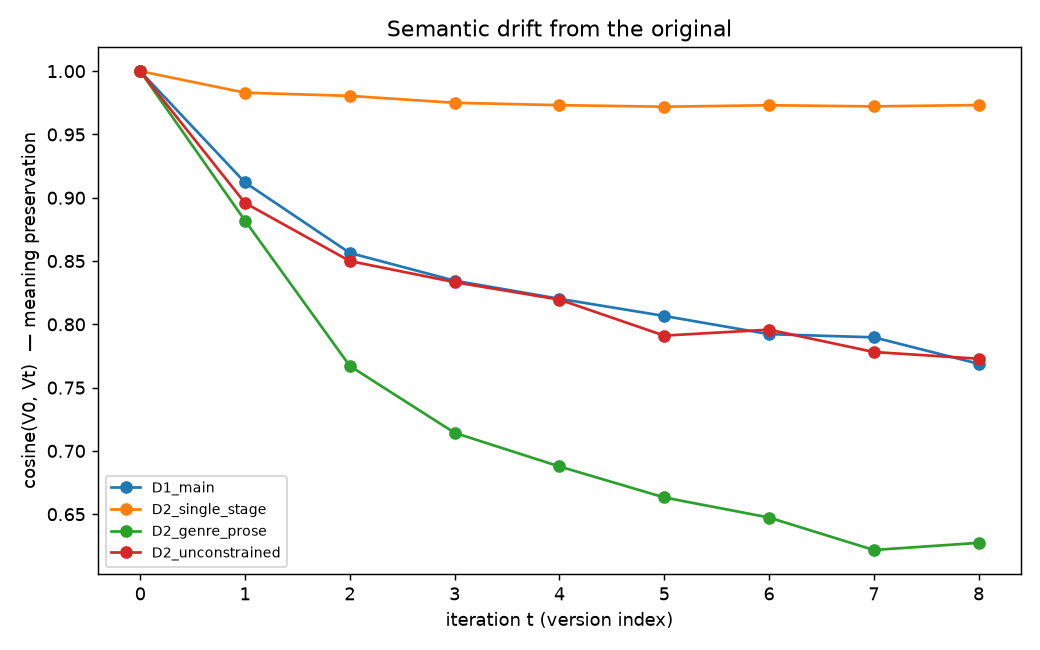
\includegraphics[width=\textwidth]{figures/semantic_drift.png}
        \caption{Semantic drift}
        \label{fig:drift}
    \end{subfigure}\hfill
    \begin{subfigure}[b]{0.32\textwidth}
        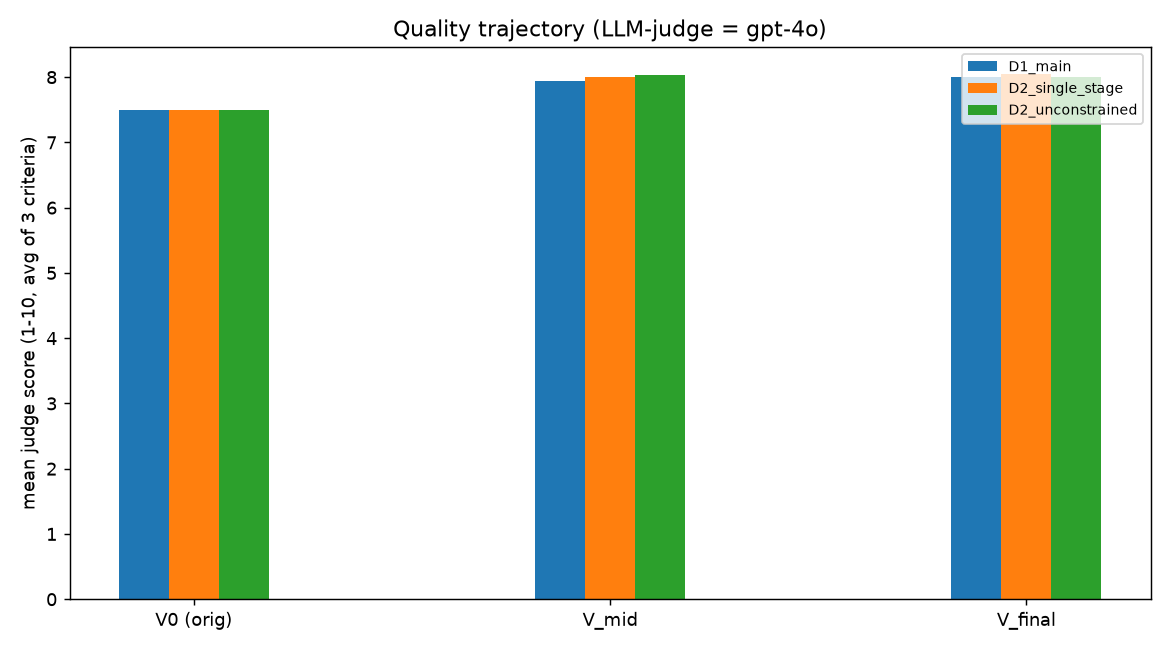
\includegraphics[width=\textwidth]{figures/quality_trajectory.png}
        \caption{Isolated quality}
        \label{fig:quality}
    \end{subfigure}
    \caption{The failure mechanism. \captiona\ Two-stage loops inflate document length
    $\sim 7\times$ over 8 iterations while the single-stage baseline holds length.
    \captionb\ Cosine similarity to $V_0$ falls (from $0.97$ single-stage to $0.77$ for
    \texttt{D1\_main}): the document drifts from its source. \captionc\ Yet isolated-quality
    judge scores barely move ($7.5\to 8.0$ for \texttt{D1\_main}), so the loop looks locally
    like improvement while globally diverging.}
    \label{fig:mechanism}
\end{figure}

\para{Inflation breaks fidelity.} \tabref{tab:fidelity} shows that inflation, not
refinement, dominates. Cosine similarity to $V_0$ falls from $0.973$ (single-stage) to $0.769$
(\texttt{D1\_main}) and as low as $0.627$ (prose; \figref{fig:drift}), while LLM-judged
meaning preservation drops from $10.0$ to $6.2$ and the loop fabricates $\sim 4$ new claims
per document (up to $15.5$ for prose). \textbf{Yet isolated-quality scores barely move}
(\figref{fig:quality}): \texttt{D1\_main}'s average of clarity, conciseness, and precision goes
$7.50\to 8.00$ from $V_0$ to $V_\text{final}$---essentially flat and slightly \emph{up}---even
as meaning preservation collapses and claims are invented. An LLM-judge scoring documents in
isolation is blind to fidelity drift: the loop feels like improvement while diverging from the
source, the self-bias / feedback-friction signature.

\subsection{Qualitative example}
\label{sec:qualitative}

The abstract \texttt{abs\_000} illustrates the mechanism concretely. $V_0$ (1617 characters)
is a dense, single-paragraph arXiv abstract on a ``capability-driven data infrastructure'' for
image generation. $V_8$ (10479 characters) is a multi-section mini-paper with invented
scaffolding---headings such as ``Key Concepts and Definitions,'' bulleted term glossaries,
operational definitions, and examples---none of which were in the original. The review that
drove the final step ($R_7$) reads: \emph{``some definitions $\dots$ could be more precise
$\dots$ provide concrete examples for less intuitive terms $\dots$ streamline sections to
avoid redundancy.''} Each round the reviewer finds fresh, legitimate-sounding gaps; each round
the reviser fills them by \emph{adding} material. There is no state in which the reviewer
returns ``no changes needed,'' so the loop cannot reach a fixed point.
